\documentclass{article}
\usepackage{graphicx}
\usepackage{fancyhdr}
\usepackage[margin=2.5cm]{geometry}
\usepackage{array}
\usepackage{longtable}


\title{The Only Way To Improve Your Edge: Daily Journals for (EURUSD)}
\author{MR5OBOT \\ \textit{"It starts with hard work, but it ends with smart work."}}
\date{\today}

\begin{document}
\maketitle
\pagestyle{fancy}
\tableofcontents
\footnote{Special thanks to [Michael J. Huddleston] or simply ICT, for Making the Path in this jungle.}
\footnote{And Thanks to [Adame Moustaine], [AM trades], [DEV] For making this notes possible.}
\newpage

% --------------------------------------------------------------------------------------
\section{Daily Bias}
\subsection{Market Maker Model Notes:}
\subsubsection{Perspectives}

\begin{center}
  \textit{\---------------------------------------------------- perspectives: \----------------------------------------------------}
\end{center}

\begin{itemize}
   \item LTP =\ Long term perspective (The Why)
    \item ITP =\ Intermediate term perspective - (The How)
    \item STP =\ Short term perspective (The Entry | KillZone)
\end{itemize}
% --------------------------------------------------------------------------------------

\subsubsection{Time-Frame Alignement} 
  
\begin{center}
  \textit{\---------------------------------------------------- Time-Frame Alignement: \----------------------------------------------------}
\end{center}

\begin{minipage}{0.34\textwidth}
    \centering
    \renewcommand{\arraystretch}{1.5} % Adjust row padding
    \begin{tabular}{|c|c|}
    \hline
      LTP (The Why)  & Monthly \\ \hline
      ITP (The How)  & Daily \\ \hline
      STP (The Entry)& 1H \\ \hline
    \end{tabular}
\end{minipage}
\hfill
\begin{minipage}{0.3\textwidth}
    \centering
    \renewcommand{\arraystretch}{1.5} % Adjust row padding
    \begin{tabular}{|c|c|}
    \hline
      LTP (The Why)  & Weeky \\ \hline
      ITP (The How)  & 4H \\ \hline
      STP (The Entry)& 15M \\ \hline
    \end{tabular}
\end{minipage}
\begin{minipage}{0.3\textwidth}
    \centering
    \renewcommand{\arraystretch}{1.5} % Adjust row padding
    \begin{tabular}{|c|c|}
    \hline
      LTP (The Why)  & Daily \\ \hline
      ITP (The How)  & 1H \\ \hline
      STP (The Entry)& 5M \\ \hline
    \end{tabular}
\end{minipage}
\hfill
\newpage

\subsection{Weekly Profiles}
Weekly profiles provide daily bias. Understanding the various ways the weekly range forms is the key for knowing when to trade establishing bias, anticipatin expansions, and mush more. All other concepts withing the trading system fall throught without this foundational knowledge.

  \begin{center}
    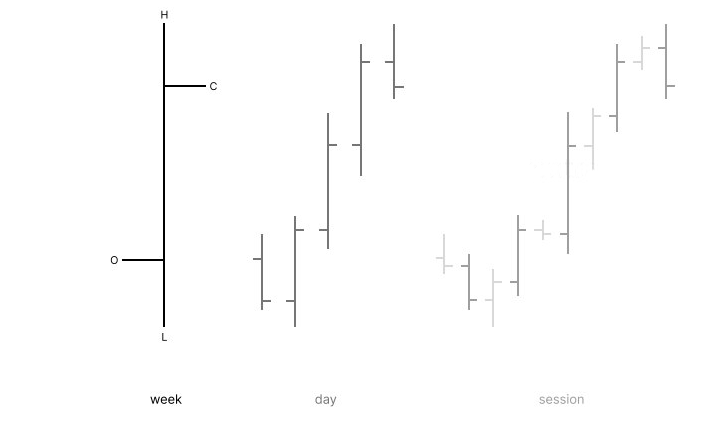
\includegraphics[width=1\textwidth]{./figures/w-profiles.png}
  \end{center}
  % \caption{}\label{fig:}
\begin{flushleft}
This paragraph is aligned to the left.
\end{flushleft}
\newpage

\section{Bias Confirmation}
\subsection{Daily Profiles}

% --------------------------------------------------------------------------------------

\newpage
\section{The Journal} 
\subsection{The Logs}

% --------------------------------------------------------------------------------------
\subsection{Charts}
\subsubsection{LTP Chart}
\subsubsection{ITP Chart}
\subsubsection{STP \textit{(The KillZone \& Entry)}}

% --------------------------------------------------------------------------------------
\newpage
\section{Summary}
\subsection{Trades Outcome}
\subsection{Notes:}

% --------------------------------------------------------------------------------------

\end{document}
